\documentclass[10pt,twocolumn]{article}

\usepackage{microtype}
\usepackage{graphicx}
\usepackage{booktabs}
\usepackage{multirow}
\usepackage{float}
\usepackage[hidelinks]{hyperref}
\usepackage[letterpaper,margin=0.75in]{geometry}
\usepackage[authoryear,round]{natbib}
\usepackage{amsmath,amssymb,amsthm}
\usepackage{tikz}
\usetikzlibrary{positioning,arrows.meta,fit,backgrounds,calc,shapes.multipart,patterns}
\usepackage{pgfplots}
\pgfplotsset{compat=1.17}
\usepackage{xcolor}
\usepackage[capitalize,noabbrev]{cleveref}

\newcommand{\todo}[1]{\textcolor{red}{[#1]}}
\newcommand{\sys}{Repowire}
\newcommand{\code}[1]{\texttt{#1}}

\tikzset{
  box/.style={draw, rounded corners=2pt, align=center, font=\scriptsize, inner sep=3pt, minimum height=0.55cm},
  st/.style={draw, rounded corners=6pt, align=center, font=\scriptsize, inner sep=3pt, minimum height=0.5cm, minimum width=1.2cm},
  arr/.style={-{Latex[length=1.8mm]}, thick},
  lbl/.style={font=\tiny, align=center, fill=white, inner sep=1pt},
}

\title{Repowire: Experience with Addressing and Delivery\\in a Persistent Coding-Agent Mesh}
\author{Prassanna Ganesh Ravishankar\\Independent Researcher\\\texttt{me@prassanna.io}\\\todo{co-author line}}
\date{16 October 2026. Working draft for arXiv and workshop review.}
\begin{document}
\maketitle
\begin{abstract}
Task-scoped coding-agent workflows delegate work from a parent to temporary workers within one tool. Repowire instead treats coding agents as persistent, directly addressable peers across runtimes and repositories, with humans participating through the same protocol. We report experience with a daemon that maintains this mesh through reconnects and runtime changes. A retrospective audit finds substantial registration churn and stale journal state around restarts. A small residual of address-key collisions is consistent with sibling sessions sharing a folder; its size is stable under two interval sensitivities. Operational records illustrate why runtime evidence matters during eviction and why explicit failure receipts matter during delivery. Cross-runtime exchanges and human use through Telegram show that the communication paths are used. The journal does not measure a benefit from carrying context across tasks. Missing registration evidence prevents replaying identity decisions or establishing session continuity.
\end{abstract}

\section{Introduction}
\label{sec:intro}

A task-scoped coding workflow starts with an orchestrator that delegates work to subagents, optionally in separate git worktrees, and collects their results. The parent holds the task context and decides what survives the workers' completion. Claude Code documents this delegation pattern and worktree isolation \citep{subagents2026}. It organizes parallel work within a task; our concern is communication among repository sessions that remain useful across tasks.

\sys{} treats those sessions as directly addressable peers. A peer can ask another peer without routing the exchange through a parent or asking a human to relay it. Peers may use different runtimes and work in different repositories; relay clients can connect from another machine. The human is also a peer, reachable through a phone or browser. The intended lifetime of a peer's role and context extends beyond one task, although its process and registration may change.

\paragraph{Task tree and persistent mesh.}
The contrast is between two organizational patterns: a task tree whose workers return results to their parent, and a mesh whose peers communicate directly across successive tasks. A task tree can stay within one runtime; the mesh connects heterogeneous runtime sessions. These patterns compose: a peer can use its runtime's subagent fan-out internally. They are not exclusive product categories. Claude Code supports subagent resumption and messaging between named subagents; Agent Teams supports direct teammate communication \citep{subagents2026,agentteams2026}. We do not measure which pattern is dominant or compare their task performance.

\sys{} runs as a daemon on the developer's machine. Agent sessions register as peers, and runtime bridges deliver messages through native input interfaces. Telegram, Slack and web control surfaces register with the \code{human} role. An orchestrator coordinates work through the same message protocol as other peers.

The design changed in response to operational failures. Early versions routed by display name and terminal pane. The operator's notes record stale registrations and messages delivered to the wrong session. We describe the mechanisms introduced to address these failures and use the journal to measure the resulting deployment.

\paragraph{Contributions.}
The experience raises two questions: what identity cost comes with keeping peers addressable across tasks, and what communication paths are used? We describe the identity and delivery mechanisms developed in this deployment (\cref{sec:design}), and audit the ambiguity that alternative address keys would introduce in its retained records (\cref{sec:eval}). We relate the operational evidence to limits of request-triggered repair and human interaction (\cref{sec:lessons}). The implementation is open source; this paper is an experience report rather than a controlled comparison of implementations.

The study covers one mesh operated by the author (\cref{sec:limits}). The journal records sender and recipient identities, request closure and registration activity. Prior studies examine coding agents through repository activity \citep{agarwal2026velocity,mazloomzadeh2026prs}, practitioner surveys \citep{pan2026measuring}, or collaborative tasks \citep{khatua2026cooperbench}. Our measurements concern a deployment used across successive tasks and sessions.

\section{Setting and Goals}
\label{sec:setting}

\paragraph{The operator's situation.}
One developer maintains several repositories (a product, its infrastructure, a few libraries, a website) and runs a coding agent in each. The agents are on different runtimes because the runtimes have different strengths and separate usage quotas. Work arrives from a phone, a laptop, or a scheduled job. Sessions are long-lived in intent and short-lived in practice: terminals close, laptops sleep, runtimes are upgraded, daemons restart.

\paragraph{Goals.}
\begin{description}
\item[G1 Address.] The canonical address is a daemon-minted peer id; a display name is a human-facing alias. Reconnects should recover the id when identity evidence permits, without merging distinct live sessions. Session continuity is a goal, not an invariant established by this study.
\item[G2 Deliver.] A message to a live session reaches its native input, and the sender learns whether it did.
\item[G3 Heterogeneity.] Runtimes differ in hooks, session models and input paths; the protocol must not.
\item[G4 Humans as peers.] The person is addressable and addressed by the same primitives as agents, from a phone.
\item[G5 No polling.] Agents do not send liveness heartbeats.
\item[G6 Record.] Journal requests, replies and lifecycle decisions with enough evidence to diagnose failures. The retained records omit registration evidence and restart boundaries, so they do not yet meet this goal fully.
\end{description}
G5 follows an incident in which timer-driven reconciliation marked live peers offline. Request-triggered repair can leave stale entries until another request arrives (\cref{sec:lazy}).

\section{Design}
\label{sec:design}

\Cref{fig:arch} shows the components. The daemon is the only routing hub. Everything else, including human surfaces and the hosted relay, is a client. The identity rules below describe commit \code{880690f8} (16 October 2026), after the journal window used in the evaluation.

\begin{figure*}[t]
\centering
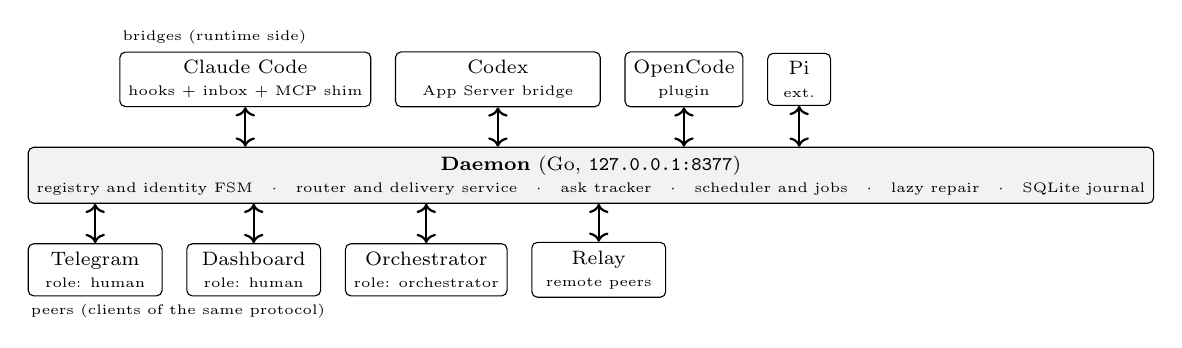
\begin{tikzpicture}[node distance=3mm]
\node[box, minimum width=2.6cm] (cc) {Claude Code\\ \tiny hooks + inbox + MCP shim};
\node[box, minimum width=2.6cm, right=of cc] (cx) {Codex\\ \tiny App Server bridge};
\node[box, minimum width=1.4cm, right=of cx] (oc) {OpenCode\\ \tiny plugin};
\node[box, minimum width=0.8cm, right=of oc] (pi) {Pi\\ \tiny ext.};
\node[box, minimum width=7.6cm, below=5mm of $(cx.south)!0.5!(oc.south)$, fill=gray!10] (d) {\textbf{Daemon} (Go, \code{127.0.0.1:8377})\\ \tiny registry and identity FSM \; $\cdot$ \; router and delivery service \; $\cdot$ \; ask tracker \; $\cdot$ \; scheduler and jobs \; $\cdot$ \; lazy repair \; $\cdot$ \; SQLite journal};
\node[box, below=5mm of d.south west, anchor=north west, minimum width=1.7cm] (tg) {Telegram\\ \tiny role: human};
\node[box, right=of tg, minimum width=1.7cm] (db) {Dashboard\\ \tiny role: human};
\node[box, right=of db, minimum width=1.7cm] (or) {Orchestrator\\ \tiny role: orchestrator};
\node[box, right=of or, minimum width=1.7cm] (rl) {Relay\\ \tiny remote peers};
\foreach \n in {cc,cx,oc,pi} \draw[arr, <->] (\n.south) -- (\n.south |- d.north);
\foreach \n in {tg,db,or,rl} \draw[arr, <->] (\n.north) -- (\n.north |- d.south);
\node[lbl, above=0.5mm of cc.north west, anchor=south west] {bridges (runtime side)};
\node[lbl, below=0.5mm of tg.south west, anchor=north west] {peers (clients of the same protocol)};
\end{tikzpicture}
\caption{Components. Bridges translate each runtime's native session API into the peer protocol; the daemon resolves peer identities before transport delivery. Human surfaces, the orchestrator and the relay are clients.}
\label{fig:arch}
\end{figure*}

\subsection{Peers, circles, roles}

A \emph{peer} is one running agent session: a display name derived from its working directory and runtime (\code{torale-codex}, suffixed on collision to \code{torale-2-codex}), a working path, a runtime (\emph{backend}), a status (online, busy, offline), a per-turn state, a free-text description the agent sets, and a last-seen time. A \emph{circle} is a routing scope that by default maps to a terminal multiplexer session, so agents started together can address each other and agents started elsewhere cannot. A \emph{role} is metadata: \code{agent} by default; \code{human} for control surfaces; \code{orchestrator} for a coordinating session; \code{service} for service clients such as the relay. Roles that bypass circles may name a circle explicitly; an ordinary agent cannot.

\subsection{Identity}
\label{sec:identity}

The daemon routes by a minted \code{peer\_id}. Addressing can resolve a display name to this id; registration also uses names and paths when reclaiming an offline peer or persisted mapping. Names collide across circles. Sibling terminals and subprocesses share paths. Runtime session ids can be reused on resume and are absent on some runtimes. The incident record includes failures involving these alternatives (\cref{sec:incidents}).

\paragraph{Registration and addressing.}
Registration and message addressing use different checks (\cref{tab:proof}). Registration first checks retirement, then looks for an existing live-process holder. For Claude Code, matching process and compatible machine, backend and path can identify that holder; Codex, OpenCode and Pi also require a matching runtime session id because one process can host several sessions. The daemon next considers a claimed \code{peer\_id} with compatible backend and path. If no id has been selected, it checks the durable binding for the backend and runtime session, subject to path compatibility. It then checks the name, circle, backend and compatible-path tuple, first among offline peers and then among persisted mappings.

Tuple reclaim adopts only a unique eligible candidate. Multiple candidates cause the daemon to mint a fresh id and journal an \code{identity\_reclaim\_ambiguous} event with the candidate ids. The fresh identity receives a distinct address when the proposed name is already held. For session-scoped runtimes, binding and tuple adoption reject candidates known to run a different session when the registrant supplies a session id. They also reject a peer whose process is alive elsewhere, including an offline record whose process still runs. Claude Code can take over a same-directory registration after the old process exits, provided the candidate remains eligible; a live sibling receives a separate, suffixed name. Addressing accepts an id or display name and rejects an ambiguous name. A daemon-minted \emph{birth certificate}, valid for 24 hours by default, authenticates the tool server's identity claim. An open renewal defect can let a long-lived Codex connection outlast its certificate; subsequent MCP calls then lose peer attribution (issue \href{https://github.com/prassanna-ravishankar/repowire/issues/494}{\#494}).

\begin{table}[t]
\caption{Identity checks by operation. These checks do not form a single ordered proof hierarchy.}
\label{tab:proof}
\centering
\footnotesize
\setlength{\tabcolsep}{3pt}\begin{tabular}{@{}p{1.6cm}p{3.1cm}p{2.5cm}@{}}
\toprule
Operation & Evidence & Effect \\
\midrule
Addressing & peer id or unambiguous name & resolves recipient id \\
Tool identity & daemon-minted birth certificate & authenticates claim \\
Local adoption & matching pane metadata and process evidence & recovers local identity \\
Registration & claimed id, session binding, or unique eligible name tuple & reuses compatible identity \\
Kill or restart & spawn ownership or pane metadata naming the peer id & authorises pane destruction \\
Mapping restore & persisted mapping & restores role, circle and description \\
\bottomrule
\end{tabular}
\end{table}

\paragraph{Lifecycle.}
\Cref{fig:lifecycle} shows the lifecycle. A clean quit, an agent-exit report, a pane takeover or three negative pane-liveness verdicts can retire an identity and sever its transport. An inconclusive verdict neither adds nor resets a strike. A soft retirement can be lifted by a live-process claim, a daemon-verified birth certificate or a compatible session binding. Tuple reclaim does not revive a retired identity. An explicit operator close creates a hard retirement that rejects reconnects claiming that id even when its process remains alive. On restart, the daemon reloads retirement records from the preceding 72 hours.

\begin{figure}[t]
\centering
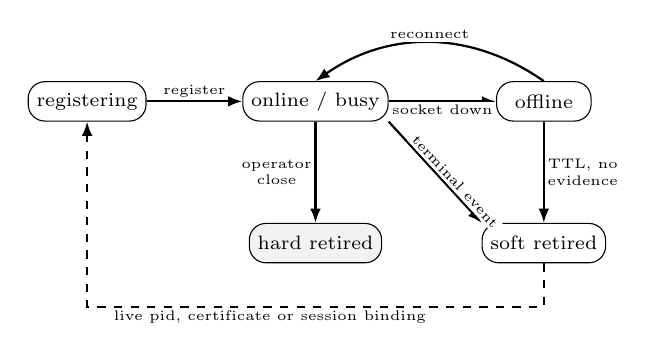
\begin{tikzpicture}[x=1cm,y=1cm]
\node[st] (reg) at (0,0) {registering};
\node[st] (on) at (2.9,0) {online / busy};
\node[st] (off) at (5.8,0) {offline};
\node[st, fill=gray!10] (hard) at (2.9,-1.8) {hard retired};
\node[st] (ret) at (5.8,-1.8) {soft retired};
\draw[arr] (reg) -- node[lbl, above] {register} (on);
\draw[arr] (on) -- node[lbl, below] {socket down} (off);
\draw[arr] (off.north) to[bend right=35] node[lbl, above] {reconnect} (on.north);
\draw[arr] (on) -- node[lbl, left] {operator\\close} (hard);
\draw[arr] (off) -- node[lbl, right] {TTL, no\\evidence} (ret);
\draw[arr] (on.south east) -- node[lbl, sloped, above, pos=0.65] {terminal event} (ret.north west);
\draw[arr, dashed] (ret.south) -- ++(0,-0.55) -| node[lbl, below, pos=0.3] {live pid, certificate or session binding} (reg.south);
\end{tikzpicture}
\caption{Go registration lifecycle. Soft retirement permits verified recovery; operator close blocks claims to the old id. Restart reloads mappings and recent retirement records, not live peers.}
\label{fig:lifecycle}
\end{figure}

\paragraph{Restart.}
The Go daemon loads durable mappings and recent retirement records at startup, but does not recreate live peers from terminal panes. Peers register when their runtime connects. The Python implementation had a pane-hydration pass; it was removed at the Go cutover and was not ported. The Go daemon still lists orphan panes for explicit linking by the operator.

\paragraph{Descriptions and sessions.}
A peer's \emph{description} is agent-set task state with no expiry; each turn is shown the current value and asked to update it. A \emph{session} is the durable context behind a peer: a binding from the daemon's session id to the runtime's own session id, which permits resume after the executor is gone.

\subsection{Message protocol}
\label{sec:protocol}

The daemon routes four message types, chosen by lifecycle rather than content.
\begin{itemize}
\item \code{ask(to, text)} is non-blocking and returns a correlation id. The recipient closes it with \code{ack(id)} (seen), \code{ack(id, reply)} (reply delivered to the asker), or \code{decline(id, reason)}. Follow-ups chain with \code{ask(reply\_to=id)}. Runtime integrations remind recipients about open asks at turn boundaries. Claude Code's Stop hook can block turn completion with a reminder when a pane id is available; OpenCode reminds on idle and Pi at a turn boundary. Prose mentions do not count as acknowledgement calls.
\item \code{notify(to, text)} is fire-and-forget with no lifecycle.
\item \code{broadcast(text)} normally reaches peers in the sender's circle and recipients whose roles bypass circles. A sender with a bypass role can reach other circles. Non-addressable peers are skipped, and human-inbox surfaces have separate delivery filtering.
\item A \emph{structured question} is an ask with a typed envelope (choice, text or acknowledge) answered through \code{answer}. Tool permission is a scope on a choice question and denies on timeout.
\end{itemize}
Peer-originated deliveries are framed so that a runtime can distinguish them from its user's instructions; messages from human surfaces are framed as user instructions. An ask to a peer the runtime says cannot accept direct input (a sub-agent thread) is refused before any state is created. Replies always reach the asker regardless of circle, because the route was fixed at ask time.

An agent explicitly closes or replies to an ask through the protocol. The daemon can also close asks on expiry, peer eviction, loss of addressability, or a job outcome. The default expiry is 24 hours. Notifications create no tracked obligation. The targeted-message UI defaults to asks; explicit syntax selects notifications.

\subsection{Bridges and transports}
\label{sec:bridges}

A \emph{bridge} translates between a runtime's session API and the peer protocol. Claude Code uses lifecycle hooks and an authenticated inbox for inbound delivery. A stdio shim supplies its identity when proxying tool calls to the daemon. Codex uses a supervised companion on the App Server socket to register threads and steer active turns. OpenCode and Pi load a plugin or extension inside the runtime. A \emph{transport} is the delivery path exposed by a bridge. Failed native delivery produces a failure receipt; the bridge does not fall back to terminal keystrokes. The router resolves a peer before passing the message to its transport.

\subsection{Lazy repair}
\label{sec:lazy}

Selected HTTP handlers, WebSocket connections and the MCP \code{list\_peers} tool trigger liveness reconciliation, at most once per 30 seconds. Other MCP tools do not trigger it. Clean quits deregister through a session-end hook. A socket supervisor reports an agent process exit, and repair checks for inconsistencies missed by these paths. The registry can therefore be stale until a request triggers repair. The daemon emits a \code{peer\_contradiction} event when it detects an inconsistency or refuses an illegal lifecycle transition. Repair deduplicates reports by peer and contradiction code. The client-side socket supervisor checks its agent process on a five-second timer; the request-triggered policy applies to daemon reconciliation, not every client activity. An operator can also request reconciliation and inspect reachability and open asks. This policy replaced timer-driven reconciliation after a spurious signal marked 43 peers offline (\cref{sec:incidents}).

\subsection{Humans and orchestrators as peers}
\label{sec:humans}

Control surfaces register with the \code{human} role, bypass circles, and use the same four message types. A message from the phone arrives at an agent as a user instruction; an agent's reply to the phone is an \code{ack} with text. Structured questions render as buttons. A \emph{human inbox} (October 2026) queues asks addressed to the human across surfaces.

An orchestrator is a peer with \code{role=orchestrator}; coordination is performed by the session. It is a long-running session the operator addresses from a phone, which scans a board, dispatches asks or durable jobs to project peers, tracks replies, requests reviews, and closes out. Its workspace holds communication preferences, project scope, and memory files; the daemon performs a bounded lexical recall over them and prefixes matching entries to inbound messages. A second orchestrator can coexist as an observer.

\subsection{Schedules, jobs, and the journal}

A \emph{schedule} delivers a future notification or tracked ask. A \emph{job} is a durable work record with an executor. In the Go implementation, dispatch uses the unregistered sender id \code{daemon-job-runner}, not a registered \code{@jobs} peer. A user-role chat event containing the work and attempt markers arms the job. The next assistant chat event from the assigned executor completes the armed work. Claude Code's Stop hook posts both events at turn end, so arming and completion can occur during the same Stop; the Codex bridge can post the user event as it occurs. A terminal executor failure closes active work with \code{executor\_died}. Only dispatch is lease-bounded; delivered work is not reaped by a clock.

The journal (G6) is an append-only event table in SQLite plus a per-message delivery-trace ledger. Trace stages record creation and recipient resolution, transport outcomes such as \code{websocket\_sent} or \code{thread\_input\_accepted}, and closure. There is no generic \code{delivered} stage. Resolved ids and status fields identify the intended recipient and recorded transport outcome. They do not independently establish which runtime session consumed the message. \Cref{sec:eval} uses this journal as the measurement instrument.

\section{Implementation}
\label{sec:impl}

\sys{} is a single Go binary (daemon, CLI, hooks, bridges, tool server, Telegram and Slack clients, relay client) with an embedded dashboard; the first eight months were Python, and the native cutover (PR \#382, 10 August 2026) splits the journal into two eras with different schemas (\cref{sec:method}). State is SQLite with versioned migrations, whose application dates on the studied host record the journal's schema changes: event journal (22 May 2026), tracked work (25 May), delivery traces (30 May), retired identities (11 June), peer provenance (18 September), routing-decision index (11 October), human inbox (13 October). A hosted relay tunnels dashboard and socket traffic so that a mesh on a home machine is operable from elsewhere; remote agents can join through a relay-side tool server. The repository is Apache-licensed. \todo{artifact URL}

\section{Deployment Evidence}
\label{sec:eval}

\subsection{Method and data}
\label{sec:method}

We use an immutable state-database backup taken on 14 October 2026 and the operator's written incident record. The journal spans 22 May to 14 October: 146 calendar days, 93 with an event and 64 with an active agent peer. The Python implementation (era A) records asks as events and some replies as notification text. The Go implementation (era B, from 10 August) records registration events and typed delivery traces. The job runner was active in era A and retired at the cutover. The workloads and measurement instruments differ.

The key audit uses era B only. Offline events do not fully record registry loss at daemon restarts; we therefore check event-only intervals against separately extracted daemon-start markers. Its script, tests and aggregate output are in \code{paper/repowire/analysis}. The private backup contains message text and is not released. Other descriptive results follow the evidence inventory's cross-era reconstruction, which excludes job-runner dispatch from human and agent request counts.

\subsection{The identity cost: address-key exposure}
\label{sec:lifecycle}

The audit asks whether an alternative key would identify more than one recorded-online peer when a delivery attempt resolved its recipient. It does not replay registration rules. All 4,203 era-B \code{peer\_online} payloads are empty, and their \code{session\_id} column repeats the peer id. The journal therefore lacks event-time process, path and runtime-session evidence needed to reconstruct identity selection.

\paragraph{Keys and coverage.}
Observed display names are outputs of the daemon's identity system: it suffixes names to distinguish live peers within a circle. They are not independent baseline keys. Event names and retained mappings agree where both exist. Only 72 of the 232 online peer ids retain circle and path metadata in \code{peer\_session\_mappings}; the backup has no \code{peers} table. Reaping, stale eviction and unregistering delete mappings. This cohort therefore has survivorship bias: 38/72 mapped peers are right-censored in the event-only reconstruction, compared with 83/232 overall. It overrepresents the stale records that inflate uncapped overlap.

We derive a default base name from the final path component and backend using \code{buildDisplayName}'s sanitization. We preserve numeric folder suffixes rather than trying to reverse the daemon's naming decisions. Preferred-name inputs are unavailable. The base, base-plus-circle and base-plus-exact-path comparisons all use the same mapped cohort, with static attributes applied retrospectively.

Backend/session keys come from final \code{session\_bindings}. Updates replace the owner of an existing binding, matched first by source URI and then by runtime session scoped to backend and project. Earlier owners can disappear from the snapshot. We also exclude 31 peers with multiple keys, leaving 171 covered peers. The resulting zero is a snapshot artifact, not a test of a session-id policy. We group it with the peer-id uniqueness control; neither establishes registration correctness. Binding creation and last-seen times are observation bounds, not assignment-validity intervals.

Earliest recipient resolution per message kind and trace id defines an attempt: 303 attempts, including 267 asks and 36 notifications. A key is known for all 303 attempts under observed names, for 134 under mapped keys, and for 112 under backend/session. Eligibility additionally requires an observed target interval. Missing target intervals are unknown, not orphaned deliveries; missing competitor keys reduce coverage.

\paragraph{Interval sensitivities.}
The event-only reconstruction opens an interval on \code{peer\_online}, closes it on offline or reaped, and leaves repeated online events within an open interval unchanged. Intervals are half-open. This gives 499 intervals for 232 peer ids, of which 83 remain open at the window end. We compare three treatments (\cref{tab:exposure}):
\begin{enumerate}
\item \emph{Last-observation cap} (primary): cap each interval at that peer's latest timestamp in the event or delivery-trace peer-id column. This removes silent tails, but a recorded association is not independent proof of process liveness.
\item \emph{Restart closure}: close all registry intervals at each daemon start, then rebuild from the raw lifecycle events. Later online events reopen intervals. We use 64 Go start markers from the daemon log, interpreting its naive timestamps in the host's Europe/London zone (UTC+1 throughout the window). The offset was checked against same-peer journal observations. This gives 936 intervals and 13 right-censored ids.
\item \emph{Uncapped}: retain open intervals to the last journal event. This is the stale-record upper scenario, not an estimate of live concurrency.
\end{enumerate}

Restart closure preserves all 298 eligible observed-name attempts and all 131 mapped-key attempts. Seventy of the 83 originally right-censored ids acquire a restart boundary. This exposes missing lifecycle boundaries in the journal, not evidence of traffic without re-registration. Simply clipping an already-merged interval at its first restart would discard later online events and give the wrong denominator. The artifact also reports a UTC interpretation of the log as a timezone sensitivity.

\begin{table}[t]
\caption{Exposure sensitivity. Peers is key coverage out of 232; eligible attempts have an observed target interval. The last-observation cap and restart rebuild preserve the listed eligibility. The last three columns count potential ambiguity, not misdelivery. Snapshot controls are not policy comparisons.}
\label{tab:exposure}
\centering\scriptsize
\setlength{\tabcolsep}{2.7pt}
\begin{tabular}{@{}lrrrrr@{}}
\toprule
key & peers & eligible & cap & restart & uncapped \\
\midrule
observed name & 232 & 298 & 0 & 0 & 66 \\
observed name + circle & 72 & 131 & 0 & 0 & 0 \\
observed name + path & 72 & 131 & 0 & 0 & 50 \\
base name & 72 & 131 & 4 & 4 & 83 \\
base + circle & 72 & 131 & 4 & 4 & 7 \\
base + path & 72 & 131 & 4 & 4 & 83 \\
\midrule
backend + session & 171 & 110 & 0 & 0 & 0 \\
peer id & 232 & 298 & 0 & 0 & 0 \\
\bottomrule
\end{tabular}
\end{table}

\paragraph{Residual and concentration.}
The base-name sensitivity range is [4, 83] exposures among 131 eligible attempts; the observed-name range is [0, 66] among 298. These are heuristic scenarios, not statistical bounds on true concurrency. Both sensitivities retain the same four base-name exposures. In each, a competing id shares the target's path and circle but has a different observed display name. The residual is consistent with sibling concurrency distinguished by daemon suffixing; it does not establish misdelivery.

The uncapped base exposures involve nine targets and seven keys. The base key \code{orchestrator-claude-code} contributes 47 of 83, and the corresponding observed name contributes 47 of 66. Uncapped counts are therefore dominated by stale-record exposure and concentrated in one name. They do not support a claim that ambiguity was common among live sessions.

Aggregate pair-overlap duration is equally sensitive. For base names it is 61.18 pair-days with the last-observation cap, 115.76 with restart closure and 2,347.22 uncapped. Pair-days sum overlap over unordered pairs, not elapsed wall time. Reuse is distinct from concurrency: 41 of 136 observed-name keys and 14 of 27 derived base keys accumulate multiple peer ids over the window. This does not identify session splits. The artifact retains pair and set counts for each treatment.

Twenty-one peer/timestamp groups contain both opening and closing events with unknown order. The main reconstruction closes the interval and waits for the next unambiguous online event. Ordering online last instead leaves the uncapped exposure counts unchanged. The interval sensitivities address a larger uncertainty than these timestamp ties.

\paragraph{Address versus alias.}
Across the full journal, the name \code{repowire-claude-code} appears with 49 peer ids. The orchestrator class contains 137 distinct registration identities, not 137 re-registrations of one demonstrated runtime session. These observations motivate separating aliases from addresses. They neither prove nor refute continuity of an individual session. Recovering the same peer id after resume remains a separate implementation obligation (\cref{sec:limits}).

\subsection{Runtime evidence and lazy repair}
\label{sec:repair-evidence}

The journal records 706 \code{offline\_peer\_still\_has\_runtime\_evidence} decisions across 33 distinct peer ids. At these decisions, a naive TTL policy without the runtime-evidence check would have proceeded to eviction. This is a one-decision counterfactual: repeated observations of the same peer are not independent prevented evictions, and an earlier eviction would change the later event stream.

Across both eras, recorded offline reasons include 226 clean \code{session\_end} events and 32 \code{transport\_failure} events. Other reasons include missing panes and agent exits. These records show that lifecycle hooks provide a path to update liveness without agent heartbeats (G5). They do not measure detection delay or establish that lazy repair is preferable under every workload. The journal lacks independent death times for such a comparison.

\subsection{What the mesh supports}
\label{sec:closure}\label{sec:traffic}\label{sec:hetero}

\paragraph{Visible outcomes.}
Five ask traces close with \code{send\_failed}. These are visible delivery-failure outcomes, not successful task completions. The distinction matters when interpreting closure: an ask can close because the daemon reports that delivery failed.

Recorded closure is 909/1,040 (87.4\%) in era A and 260/265 (98.1\%) in era B for non-machine asks. Of the combined 1,169 close records, 855 depend on parsing era-A notification text. Era B uses typed events, and the workload also changes at the cutover. We retain these fractions as descriptions of the records, not an estimate of a reliability improvement. A close or acknowledgement does not establish task completion; missing closes do not identify a particular failure mechanism.

\paragraph{Human participation.}
Human surfaces originate 698 of 1,305 non-machine asks (53.5\%), but only seven asks go from agents to humans. The common protocol therefore carries substantial human-initiated work without showing much agent-initiated consultation. Notification counts are not evidence of human intent: the targeted-message UI defaults to an ask and requires explicit syntax for a notification.

Of the 698 human-origin asks, 680 come through Telegram and 18 through the dashboard; none come through Slack. Telegram supports phone use, but the journal identifies the service rather than the physical device.

\paragraph{Cross-runtime exchanges and initiation.}
Of 591 agent-to-agent asks, 307 (52\%) cross runtimes; 281 of these are between Claude Code and Codex. This demonstrates use of the bridges, not improved task quality. Of 348 peer-to-peer asks, about 220 have no recorded dispatch to the sender in the preceding 30 minutes, falling to 184 with a two-hour window. The proxy includes human, orchestrator and machine asks, their notifications (events and resolved notify traces), and assigned-job state events. This is consistent with agent-initiated requests, but status notifications need not dispatch work, and earlier or unrecorded dispatch is invisible. The eight relay-origin asks show use of the remote entry point; they do not establish a distribution of work across machines.

Recipient repetition is treated in the companion routing study \citep{routerpaper2026}; the artifact supplies peer-only repetition, gap splits and a per-sender recipient-frequency null rather than using pooled human traffic as evidence of persistence.

\subsection{Operational failures}
\label{sec:incidents}

The operator's notes describe phantom registrations, wrong-recipient delivery, dropped replies and state lost across daemon restarts. Configuration drift also caused the installed executable to differ from the checkout. We use these cases to explain design changes rather than estimate failure frequencies. \Cref{app:incidents} gives examples. The evidence inventory links note incidents to journal or daemon-log signatures, including the mass-offline incident that motivated removing periodic reconciliation.

MAST describes failures in multi-agent execution traces \citep{cemri2025mast}. A dropped reply can resemble withholding information, but that label alone does not identify a closed request or failed transport as the cause. Lifecycle evidence is needed to distinguish these cases. \todo{Validate the incident-level MAST coding; the evidence inventory contains class counts, not a coding audit.}

\section{Lessons}
\label{sec:lessons}

\paragraph{Separate address selection from alias resolution.}
Registration churn and stale records dominate the identity evidence. A small residual of shared-base-name exposures remains under both interval sensitivities, consistent with sibling concurrency. Canonical peer ids let the daemon record a specific intended recipient. Registration still has to decide whether a reconnect belongs to that identity; unique ids alone cannot make that decision correct.

\paragraph{Preserve evidence at the decision point.}
Retained mappings recover only part of the population and are not historical registration inputs. Recording the identity rule and its inputs when registration occurs would permit future policy replay. Restart loss also needs an explicit journal boundary: the event-only reconstruction leaves 83 ids open, whereas rebuilding with daemon starts leaves 13. The current audit cannot recover misbinds or session splits.

\paragraph{Check runtime evidence before expiry.}
The spared-event records show decisions at which a TTL alone would discard an identity that still had runtime evidence. Request-triggered repair avoids continuous liveness polling but leaves stale registry state until another request or lifecycle event arrives. A useful next measurement is the delay from independently observed process death to registry repair.

\paragraph{Distinguish addressability from consultation.}
Human endpoints are widely used to initiate work, while agent-to-human asks are rare in this deployment. Exposing a human peer does not by itself produce a workflow in which agents seek human input.

\paragraph{Feasibility is not a measured persistence benefit.}
Cross-runtime requests and Telegram participation demonstrate usable communication paths. Pairs recur across UTC days at the alias level: 11 of 89 observed-name pairs, carrying 134 of the 348 peer-to-peer asks. At the registration level, only four of 114 peer-id pairs recur. Churn splits relationships across registrations, while alias reuse can join different sessions. Neither measure establishes that context carried over or identifies task boundaries. The deployment therefore supports the feasibility of the mesh and documents its identity costs; a task-level study is needed to measure whether persistence improves work.

\section{Related Work}
\label{sec:related}

\paragraph{Task-spawned multi-agent frameworks.}
CAMEL, MetaGPT, ChatDev, AutoGen and OpenHands study coordination among agents within an application or task \citep{li2023camel,hong2024metagpt,qian2024chatdev,wu2023autogen,openhands2024}. MAST analyses failures in multi-agent execution traces \citep{cemri2025mast}. Our incident record concerns a deployment across successive sessions, including registration and delivery failures. \todo{Check the framework comparison against supported persistence and human-interaction features.}

\paragraph{Coding-agent fleets.}
Claude Code Agent Teams uses a lead session and teammate sessions with shared tasks and messaging; its documentation lists in-process teammate resumption as a limitation \citep{agentteams2026}. Gastown separates worker identities from sessions and provides lifecycle supervision \citep{gastown2026}. Cursor reports contention and coordination failures in a shared-file design before introducing separate planners and workers \citep{cursor2026}. \sys{} routes messages across runtimes and admits human control surfaces as peers.

\paragraph{Protocols.}
\sys{} exposes tools to runtimes through MCP. Interoperability surveys describe discovery and task exchange through MCP, ACP, A2A and ANP \citep{ehtesham2025survey,mcp2025survey}. Our design concerns the local registration evidence and runtime input paths required to deliver messages to coding sessions. \todo{Compare lifecycle and delivery semantics against versioned protocol specifications.}

\paragraph{Measurement.}
Pan et al.\ \citep{pan2026measuring} study deployed agents through interviews and a practitioner survey. Repository studies examine agent contributions and their evolution \citep{agarwal2026velocity,mazloomzadeh2026prs,msr2026survival}. CooperBench evaluates collaboration between coding agents \citep{khatua2026cooperbench}. Our journal records communication and registration activity in one deployment; it does not measure task quality. The companion paper discusses routing and delegation benchmarks \citep{decisionbench2026,orchbench2026,routerbench2024}.

\paragraph{Persistent state.}
InfiAgent reconstructs context from file-backed state \citep{infiagent2026}, while Omri et al.\ characterise agent memory systems \citep{agentmemory2026}. \sys{} stores orchestrator memory and runtime session bindings outside the current prompt. The learned-recall experiment is reported separately.

\section{Limitations and Future Work}
\label{sec:limits}

The author operates the only mesh studied. Its workload and incident notes are not a population sample. The key audit uses retrospective static attributes and censored registry intervals. It measures exposure to ambiguity, not actual misdelivery. Missing registration inputs prevent replaying the shipped identity rules; missing runtime-consumption evidence prevents identifying orphaned deliveries. Unjournaled restart boundaries inflate event-only intervals. Issue \href{https://github.com/prassanna-ravishankar/repowire/issues/493}{\#493} proposes registration-decision evidence and daemon-run identifiers. Certificate expiry without renewal can also leave long-lived Codex MCP calls unattributed (\href{https://github.com/prassanna-ravishankar/repowire/issues/494}{\#494}). The private backup cannot be released; aggregate results, analytical code and synthetic tests accompany this draft. \todo{artifact release}

Identity continuity still depends on registration order. A PID-only registration can mint a new peer before the session-start hook supplies the runtime session id. The later registration can select that live-process holder before consulting the durable session binding, so resume does not always recover the earlier peer id (issue \href{https://github.com/prassanna-ravishankar/repowire/issues/474}{\#474}). The ambiguity fix in commit \code{880690f8} postdates the journal window. The address-key audit does not evaluate that fix.

Controlled fault injection is future work. Tests should cover a pane exiting during an ask, daemon restart with an open request, session resume, sibling terminals sharing a path and expired credentials. Independent process-death timestamps would support a staleness study. We have not measured daemon CPU, memory overhead or a controlled delivery-latency baseline.

\section{Conclusion}

\sys{} connects coding-agent peers through a common request protocol across runtimes and human control surfaces. The deployment records frequent identity churn and missing restart boundaries. A small residual of same-folder sibling exposure survives two interval sensitivities; the much larger uncapped counts mostly reflect stale records. Cross-runtime exchanges and Telegram use establish communication feasibility. The journal does not establish a benefit from persistent context, which requires a task-level study.

\section*{Acknowledgements}
\todo{Acknowledge the model vendors whose agents are the peers; the review bots.}

\bibliography{refs}
\bibliographystyle{plainnat}

\newpage
\appendix
\onecolumn

\section{Incident examples}
\label{app:incidents}

One incident per class from the written record, dated by note text.
\begin{itemize}
\item \textbf{Peer leak or phantom} (2026-05-15): an ack from a retired orchestrator registration, absent from the peer list, arrived as a live request to merge an already-merged pull request.
\item \textbf{Misroute} (2026-05-14): during co-orchestration, a project peer received three of its last four asks intended for others, and a reply addressed to a suffixed name fell back to broadcast. Fixed by the reconnect identity check.
\item \textbf{Delivery drop} (2026-05-11): a reply sent on an already-closed ask returned success and was not delivered.
\item \textbf{Daemon restart disruption} (2026-05-10): repeated restarts during installer testing cleared in-memory ask state; stale reminders surfaced and pane kills were refused for pre-restart peers.
\item \textbf{Config drift} (2026-05-19): the installed CLI lacked a command present in the checkout; a forced reinstall left stale packages.
\item \textbf{Job or schedule} (2026-06-11): a job fire never armed because the executor's turn carried no marker; the fire stayed delivered.
\item \textbf{Auth expiry} (2026-06-04): a workspace token rotated to a scopeless state; after re-authentication a stale cache kept calls failing.
\item \textbf{Other} (2026-05-15): one peer wrote files into another peer's worktree and switched its branch.
\end{itemize}

\end{document}
